% **************************************************
% Document class
% **************************************************

\documentclass[
	a4paper,
	12pt,
	bibtotoc,
	listof=totoc,
	titlepage,
	parskip=half
]{scrartcl}


% **************************************************
% Settings
% **************************************************

\usepackage{settings}


% **************************************************
% Variables
% **************************************************

\newcommand*{\getUniversity}{Hochschule für angewandte Wissenschaften München}
\newcommand*{\getFaculty}{Fakultät für Informatik und Mathematik}
\newcommand*{\getTitle}{Entwurf und Bereitstellung von Microservices mit Kubernetes am Beispiel eines CRM-Systems}
\newcommand*{\getAuthor}{Simon Hirner}
\newcommand*{\getMatriculationNumber}{02607918}
\newcommand*{\getCourse}{Wirtschaftsinformatik}
\newcommand*{\getDoctype}{Bachelorarbeit}
\newcommand*{\getSupervisor}{Prof. Dr. Torsten Zimmer}
\newcommand*{\getSubmissionDate}{04.02.2022}


% **************************************************
% PDF Metadata
% **************************************************

\hypersetup{
	pdftitle = \getTitle,
	pdfauthor = \getAuthor,
	pdfsubject = \getDoctype
	pdfkeywords = {Microservices, Kubernetes, DevOps}
}


% **************************************************
% Content
% **************************************************

\begin{document}

\titlehead{
	\begin{flushright}
		
\includegraphics[width=50mm]{logos/university_logo}
	\end{flushright}
	\begin{center}
		{\Large \getUniversity}\\
		{\large \getFaculty}
		\vspace*{10mm}
	\end{center}
}

\subject{\getDoctype\ zum Thema:}

\title{\vspace{-10mm} \getTitle}

\subtitle{Zur Erlangung des akademischen Grades Bachelor of Science}

\author{}

\date{}

\publishers{
	\parbox{\textwidth}{
		\vspace*{35mm}
		\large
		\begin{tabularx}{0.8\textwidth}{lX}
			\textbf{Vorgelegt von:} & \getAuthor \\[0.7em]
			\textbf{Matrikelnummer:} & \getMatriculationNumber \\[0.7em]
			\textbf{Studiengang:} & \getCourse \\[0.7em]
			\textbf{Betreuer:} & \getSupervisor \\[0.7em]
			\textbf{Abgabedatum:} & \getSubmissionDate \\[0.7em]
		\end{tabularx}
	}
}\normalsize

\maketitle

\begin{abstract}

\section*{Zusammenfassung}
Bei immer mehr moderne Webanwendungen findet das Architekturmuster der Microservices anwendung. Dieser Trend verändert nicht nur den Entwurf und die Implementierung von Anwendungen, sondern hat auch erhebliche Auswirkungen auf die Bereitstellung und den Betrieb. \\

In dieser Bachelorarbeit wird der Entwurf und die Bereitstellung von Microservices mithilfe von Kubernetes analysiert. \\

\end{abstract}
\begin{abstract}

\section*{Abstract}
Bei immer mehr moderne Webanwendungen findet das Architekturmuster der Microservices anwendung. Dieser Trend verändert nicht nur den Entwurf und die Implementierung von Anwendungen, sondern hat auch erhebliche Auswirkungen auf die Bereitstellung und den Betrieb. \\

In dieser Bachelorarbeit wird der Entwurf und die Bereitstellung von Microservices mithilfe von Kubernetes analysiert. \\

\end{abstract}

\addtocontents{toc}{\protect\thispagestyle{empty}}
\tableofcontents

\clearpage
\pagenumbering{Roman}
\setcounter{page}{1}
\thispagestyle{plain}
\listoffigures

\clearpage
\thispagestyle{plain}
\listoftables

\clearpage
\thispagestyle{plain}
\lstlistoflistings

\clearpage
\thispagestyle{plain}
\section*{Abkürzungsverzeichnis\markboth{Abkürzungsverzeichnis}{}}
\addcontentsline{toc}{section}{Abkürzungsverzeichnis}

\begin{acronym}

\acro{USD}{US-Dollar}
\acro{CRM}{Customer-Relationship-Management}
\acro{UNIX}{Uniplexed Information and Computing Service}
\acro{SOA}{Serviceorientierte Architektur}
\acro{API}{Application Programming Interface}
\acro{CI}{Continuous Integration}
\acro{CD}{Continuous Delivery}
\acro{DDD}{Domain-driven Design}
\acro{UI}{User Interface}
\acro{REST}{Representational State Transfer}
\acro{HTTP}{Hypertext Transfer Protocol}
\acro{URI}{Uniform Resource Identifier}
\acro{DNS}{Domain Name System}
\acro{CLI}{Command Line Interface}
\acro{HTML}{Hypertext Markup Language}
\acro{JSON}{JavaScript Object Notation}
\acro{B2C}{Business-to-Customer}

\end{acronym}	

\clearpage
\pagenumbering{arabic} 
\section{Einleitung}

Diese Arbeit wurde im Rahmen des Seminars DevOps und Cloud Computing bei Prof. Dr. Torsten Zimmer an der Hochschule München erstellt. Die Arbeit befasst sich mit der Konfiguration einer CI/CD-Pipeline mit Kubernetes. \\

Pro Woche startet Google nach eigenen Angaben über zwei Milliarden Container. Von Gmail bis YouTube laufen beinahe alle Dienste in Containern. Containertechnologien befinden sich in den letzten Jahren zweifelsfrei auf einem Siegeszug. Die Idee Software in standardisierte Pakete zu verpacken revolutionierte den Einsatz und die Distribution von Anwendungen. Um die große Anzahl an Containern zu verwalten wurden Anwendungen zur Container-Orchestrierung entwickelt. \\

Doch Container-Virtualisierung war nur eine von vielen Revolutionen. Die Cloud revolutionierte die Nutzung von Computerressourcen. Mit den verteilten Systemen in der Cloud ließ sich der Betrieb immer schwerer von Architektur und der Implementierung der Systeme trennen. Es kam zu einer weiteren Revolution, dem DevOps-Ansatz, welcher das Zusammenspiel von IT-Betrieb und Softwareentwicklung maßgeblich veränderte. \\

In dieser Arbeit werden diese Revolutionen miteinander verknüpft. Es werden die Merkmale von Container-Virtualisierung, Container-Orchestrierung und DevOps erläutert und vor allem deren Synergieeffekte in der gemeinsamen Verwendung aufgezeigt. [\cite[S. 1]{hightowerKubernetesKompakte2018}]


\clearpage
\section{Theoretische Grundlagen}

In diesem Kapitel werden die grundlegenden Begriffe und Konzepte erläutert, welche wichtig für das Verständnis der Arbeit sind. Es wird zunächst der DevOps-Ansatz und das Architekturmuster der Microservices beschrieben. Im Anschluss werden die Grundlagen von Docker sowie Kubernetes erklärt.

\subsection{DevOps}

Alle der in diesem Kapitel beschriebenen Architekturmuster, Methoden und Werkzeuge lassen sich dem DevOps-Ansatz zuordnen. Um den Gesamtkontext zu verstehen, ist es deshalb sehr bedeutsam zu wissen, was DevOps bedeutet und warum es so populär ist. Wie das Kofferwort \glqq DevOps\grqq{} bereits andeutet, beschreibt er einen Ansatz für eine effektivere und stärkere Zusammenarbeit zwischen Softwareentwicklung (Development) und IT-Betrieb (Operations). Für DevOps gibt es keine einheitliche Definition. Es ist ein Überbegriff für Denkweisen, Kultur, Methoden, Technologien und Werkzeuge. Der Kundennutzen wird dabei immer in den Mittelpunkt gestellt \parencite[vgl.][S. 1]{halstenbergDevOps2020}. Das Ziel ist es die Softwarequalität zu verbessern sowie die Geschwindigkeit der Entwicklung und Bereitstellung zu erhöhen \parencite[vgl.][S. 6]{arundelCloud2019}. Um die Ziele zu erreichen, werden etablierte Methoden und Werkzeuge eingesetzt. Die einzelnen Phasen der Entwicklung und des Betriebs miteinander zu einem Prozess, der von jedem Programminkrement durchlaufen wird \parencite[vgl.][S. 63]{trempArchitekturen2021}.

\begin{figure}[H] 
    \centering
    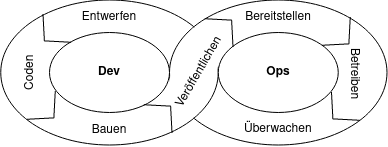
\includegraphics[width=0.75\textwidth]{figures/DevOpsKreislauf.png}
    \caption{Kreislauf und Schritte von DevOps \parencite[vgl.][S. 63]{trempArchitekturen2021}}
\end{figure}

Durch eine engere Abstimmung, Automatisierung, Continuous-Integration und Continuous-Delivery kann beispielsweise die Time-to-Market reduziert werden. Diese Kennzahl gibt an, wie lange es dauert eine Änderung zum Kunden, also auf die Produktionsumgebung, zu bringen \parencite[vgl.][S. 7]{halstenbergDevOps2020}. Auch Microservice-Architekturen und Werkzeuge wie Docker und Kubernetes können dabei unterstützen.

DevOps wird immer wichtiger, da durch das Aufkommen von Cloud Computing die Entwicklung und der Betrieb von Anwendungen nicht mehr trennbar ist. DevOps in ein Unternehmen einzuführen ist ein langwieriger Prozess. Neben der Einführung der neuen Technologien ist vor allem die Transformation der Unternehmenskultur besonders schwierig. In großen Unternehmen zeigt sich das viele Prozesse schwerfällig geworden sind und nicht mehr dem eigentlichen Kundennutzen dienen. DevOps soll dieses Problem lösen und Unternehmen wieder anpassungsfähiger machen, ohne geordnete Strukturen zu verlieren.

\begin{figure}[H] 
    \centering
    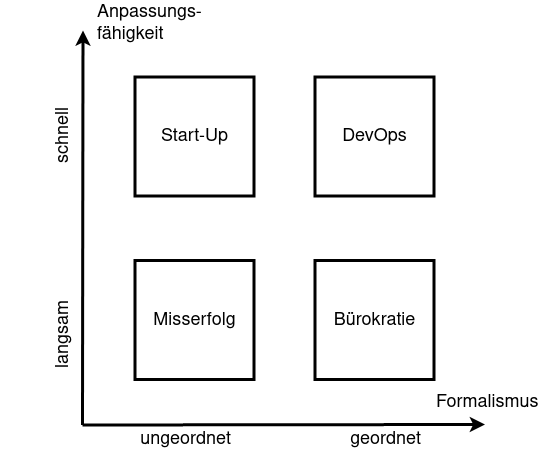
\includegraphics[width=0.7\textwidth]{figures/DevOpsKategroisierung.png}
    \caption{Kategorisierung von Unternehmen nach Anpassungsfähigkeit und Formalismus \parencite[vgl.][S. 11]{halstenbergDevOps2020}}
\end{figure}

\subsection{Microservices}

Im Mittelpunkt dieser Arbeit stehen Microservices. Bei Microservices handelt es sich um ein Architekturmuster zur Modularisierung von Software \parencite[vgl.][S. 15]{newmanMicroservices2015}. Eine einheitliche Definition für Microservices gib es nicht \parencite[vgl.][S. 2]{wolffMicroservices2018}. Bei der Beschreibung von Microservices werden Prinzipien und Merkmale einer standardisierten Definition vorgezogen. Im Folgenden werden die wichtigsten Merkmale kurz erläutert.

\subsubsection{Merkmale}

Microservices sind das Gegenteil von klassischen monolithischen Softwarearchitekturen. Ein Monolith ist eine einzelne, zusammenhängende und untrennbare Einheit. Die Erweiterbarkeit und Wartbarkeit von Monolithen ist häufig komplex, da die Codebasis umfangreich ist und mit der Zeit immer stärker wächst. Die Arbeit von mehreren Entwicklerteams ist ineffizient, da ein hoher Abstimmungsbedarf nötig ist. Des Weiteren lässt ist die Skalierbarkeit des schwergewichtigen Monolithen sehr beschränkt. Durch Modularisierung einer Anwendung lassen sich diese Probleme abschwächen, können jedoch nicht vollständig behoben werden.

\begin{figure}[H] 
    \centering
    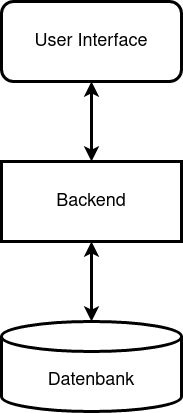
\includegraphics[width=0.2\textwidth]{figures/AufbauMonolith.png}
    \caption{Beispielhafter Aufbau einer monolithischen Architektur}
\end{figure}

Genau hier setzten Microservices an. Obwohl der Begriff Microservices noch realtiv jung ist, sind die dahinterstehenden Konzepte bereits deutlich älter \parencite[vgl.][S. 15]{newmanMicroservices2015}. Zur Verständlichkeit und leichteren Weiterentwicklung werden große Systeme schon lange in kleine Module unterteilt. Die Besonderheit von Microservices liegt darin, dass die Module einzelne Programme sind. Das Architekturmuster der Microservices zählt zu den verteilten Systemen. Die einzelnen Microservices laufen zumeist auf vielen unterschiedlichen Rechnern und kommunizieren über das Netzwerk.

\begin{figure}[H] 
    \centering
    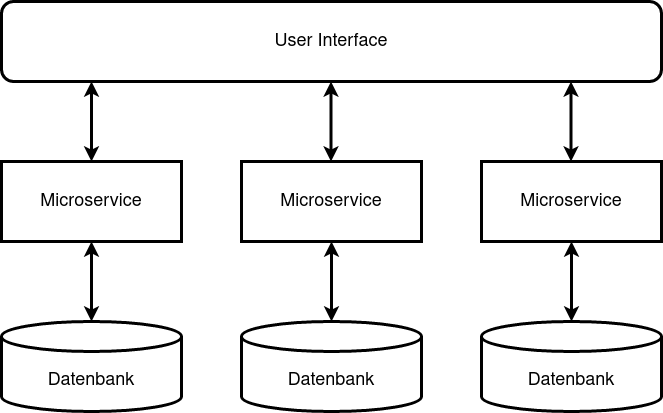
\includegraphics[width=0.71\textwidth]{figures/AufbauMicroservices.png}
    \caption{Beispielhafter Aufbau einer Microservice-Architektur}
\end{figure}

Ein einzelner Microservice soll eine Aufgabe bestmöglich erledigen. Dieser Ansatz ist angelehnt an die Philosophie von \ac{UNIX}: \glqq Mache nur eine Sache und mache sie gut\grqq{} \parencite[vgl.][]{salusQuarter1994}. Jeder Microservice bildet so eine klar definierte Funktion des Gesamtsystems ab \parencite[vgl.][S. 64]{trempArchitekturen2021}. Die Microservices müssen dabei eigenständig sein, sodass sie unabhängig voneinander verändert und bereitgestellt werden können. Die Kommunikation zwischen den Microservices erfolgt über das Netzwerk mittels sprachunabhängiger Schnittstellen, sogenannte \acp{API}. Um die Microservices unabhängig voneinander skalieren zu können, müssen sie zustandlos sein.

Die Größe eines Microservices ist nicht zwangsläufig entscheidend \parencite[vgl.][S. 2]{wolffMicroservices2018}. Der Name deutet bereits an, dass es sich um kleine Services handelt, jedoch ist eine genaue Festlegung der Größe nicht sinnvoll \parencite[vgl.][S. 22]{newmanMicroservices2015}. Eine Messung der Größe durch die Anzahl der Codezeilen wäre zwar denkbar, jedoch hängen derartige Kriterien stark von der verwendeten Programmiersprache ab. Stattdessen sollte sich die Größe an fachliche Gegebenheiten anpassen. Je kleiner die Services gestaltet werden, umso stärker kommen die in den nachfolgenden Abschnitten beschriebenen Vor- und Nachteile zur Geltung. Eine Obergrenze für die Größe eines Microservices stellt die Teamgröße dar. An einem Microservice darf immer nur ein Entwicklerteam arbeiten \parencite[vgl.][S. 23]{newmanMicroservices2015}. Kann der Microservice nicht mehr von einem Team alleine entwickelt und gewartet werden, so ist er zu groß. Ein Microservice sollte auch nur so groß sein, dass er von einem Entwickler allumfassend verstanden werden kann. Jedoch sollten Microservices auch nicht zu klein gewählt werden, da ansonsten der die Bereitstellung der vielen Microservices zu aufwendig wird.

Microservices wirken sich auf die Organisation und den Entwicklungsprozess aus \parencite[vgl.][S. 2]{wolffMicroservices2018}. Um von Microservices zu profitieren müssen Strukturen in Unternehmen überarbeitet werden. Das Gesetz von Conway besagt, dass durch die Kommunikationsstrukturen einer Organisation auch die Struktur der Systeme, welche die Organisation entwirft, vorgegeben wird \parencite[vgl.]{conwayHow1968}. Bei monolithischen Anwendungen werden die Entwicklerteams häufig nach ihrem Fachbereich aufgeteilt. Es bilden sich so beispielsweise Teams spezialisiert auf das Frontend, das Backend und die Datenbank. Die entwickelte Anwendung wird, nach dem Gesetz von Conway, auch aus diesen drei Bereichen bestehen. Wenn nun ein neues Feature umgesetzt werden soll, müssen sich alle drei Teams miteinander absprechen. Bei einer Microservice-Architektur müssen die Entwicklerteams crossfunktional mit Spezialisten aus verschiedenen Fachbereichen aufgebaut werden. Änderungen betreffen so häufig nur ein Entwicklerteam und der Koordinationsaufwand sinkt.

Häufig werden Microservices mit \ac{SOA} in Verbindung gebracht. Microservices übernehmen viele Prinzipien von \ac{SOA}. \ac{SOA} ist ein Ansatz mit dem Ziel Funktionalitäten von betrieblichen Anwendungen durch Services von außerhalb zugreifbar zu machen \parencite[vgl.][S. 2]{wolffMicroservices2018}. Ein Service bildet in diesem Kontext einen Geschäftsprozess ab. Dadurch soll Flexibilität und Wiederverwendbarkeit in der IT von Unternehmen erhöht werden. Es gibt also durchaus viele Parallelen zu Microservices, jedoch setzen sie an verschiedenen Ebenen an. Während Microservices ein konkretes Architekturmuster für ein einzelnes System ist, beschreibt \ac{SOA} wie viele Systeme in einem Unternehmens miteinander interagieren können.

\subsubsection{Vorteile}

Bei monolithischen Anwendungen, entstehen schnell unerwünschte Abhängigkeiten zwischen verschiedenen Komponenten. Die vielen Abhängigkeiten sind schwer zu überblicken und die Änderung von einer Komponente wird erschwert, da es zu unerwünschten Nebeneffekten kommen kann. In der Praxis wird so die Architektur von Monolithen mit der Zeit zunehmend schlechter \parencite[vgl.][S. 3]{wolffMicroservices2018}. Die Microservices besitzen dagegen nur eine lose Kopplung über explizite Schnittstellen. Die Hindernisse für unerwünschte Abhängigkeiten sind hier deutlich höher.

Durch die expliziten Schnittstellen ist es auch einfach einen gesamten Microservice zu ersetzten. Der neue Microservice muss lediglich die selbe Schnittstelle anbieten wie der Alte. Auch die vollständige Neuentwicklung eines Microservices ist durch die begrenzte Größe in der Regel nicht schwer. Somit können Microservices schneller an neue Technologien angepasst werden. Die Ablösung von großen Monolithen gestaltet sich dagegen häufig als eine fast unmögliche Aufgabe \parencite[vgl.][S. 29]{newmanMicroservices2015}. Darüber können Microservices auch komplett unterschiedliche Technologie-Stacks verwenden \parencite[vgl.][S. 5]{wolffMicroservices2018}. Die eingesetzten Technologien müssen dabei lediglich die entsprechende Schnittstelle anbieten können. Durch diese Freiheit kann für jeden Microservice kompromisslos die am besten geeignete Technologie ausgewählt werden.

Ein weiterer wesentlicher Grund für Microservices ist \ac{CD}. Die Microservices können unabhängig voneinander bereitgestellt werden. Tritt bei einer Bereitstellung ein Fehler auf, sind die verbundenen Risiken deutlich geringer. Es ist nicht das gesamte System davon betroffen, sondern nur der entsprechende Service. Dadurch, dass nur der veränderte Microservice neu bereitgestellt werden muss, ist die Bereitstellung schneller als bei einem Monolithen. Dadurch ermöglichen Microservices eine bessere Time-to-Market. Außerdem ist die Absicherung einer Bereitstellung, durch das parallele betreiben einer älteren Version, deutlich ressourcenschonender. Bei Monolithen wäre in so einem Fall der Ressourcenverbrauch doppelt so hoch, wie die gesamte Anwendung eigentlich benötigt.

Microservices können unabhängig voneinander skaliert werden. So kann eine einzelne Funktionalität, welcher stärker genutzt wird, einzeln hoch skaliert werden, ohne das gesamte System zu skalieren \parencite[vgl.][S. 5]{wolffMicroservices2018}]. Flaschenhälse welche eine Anwendung ausbremsen, können somit besser vermieden werden. Auch kann die Last kann durch Microservices besser verteilt werden, da sie verteilt auf unterschiedlichen Rechnern laufen können. Durch eine bestmögliche Ressourcenausnutzung können so Kosten eingespart werden \parencite[vgl.][S. 27]{newmanMicroservices2015}.

\subsubsection{Herausforderungen}

Microservices bringen neben den vielen Vorteilen auch einige erhebliche Herausforderungen mit sich. Die Aufteilung eines Systems in viele Microservices erhöht die Komplexität. Die Struktur des Systems kann mit einem schlechten Architekturmanagement schnell unübersichtlich werden \parencite[vgl.][S. 77]{wolffMicroservices2018}. Welcher Microservice eine Schnittstelle eines anderen Microservices aufruft kann von außen nicht direkt eingesehen werden. Auch auf Code-Ebene können sich ungewollte Abhängigkeiten einschleichen. Wenn mehrere Microservices beispielsweise die selbe Bibliothek verwenden, geht die lose Kopplung verloren und die Microservices können unter Umständen nicht mehr unabhängig voneinander bereitgestellt werden.

Die technologische Freiheit der Microservices kann schnell zu einer Herausforderung werden. Zu viele unterschiedliche Technologien in den Microservices erhöhen die Komplexität und den Erhalt von Fachwissen \parencite[vgl.][S.65]{trempArchitekturen2021}. Darüber hinaus wird der Wechsel von Mitarbeitern in andere Entwicklerteams erschwert.

Während Änderungen in einem Microservice sehr einfach sind gestalten sich Refactoring über mehrere Microservices hinweg als deutlich komplizierter. Bei Monolithen können Teile des Codes leicht von einer Komponente in eine Andere verschoben werden kann. Bei Microservices müssen die Teile in einen anderes  Programm verschoben werden, welches vielleicht sogar einen anderen Technologie-Stack verwendet. Die Auswirkung von Fehlentscheidungen bei der Einteilung der Microservices sind somit sehr hoch \parencite[vgl.][S. 6]{wolffMicroservices2018}.

Microservices sind verteilte Systeme und bringen auch die damit verbundenen Nachteile mit sich. Da die Kommunikation zwischen den Microservices über das Netzwerk läuft, ist die Geschwindigkeit der Microservices von der Netzwerklatenz abhängig. In der Zeit, die ein Microservice benötigt, um einen anderen Microservice aufzurufen, könnte ein moderner Prozessor Millionen von Instruktionen abarbeiten \parencite[vgl.][S. 73]{wolffMicroservices2018}. Außerdem ist Kommunikation über ein Netzwerk unzuverlässig \parencite[vgl.][S. 76]{wolffMicroservices2018}. Ausfälle von einzelnen Microservices können die Funktionalität des Gesamtsystems einschränken.

\subsubsection{Architektur}

Die Architektur von Microservices lässt sich in die Micro-Architektur und die Makro-Architektur untergliedern. Die Micro-Architektur bezieht sich auf die Architektur eines einzelnen Microservices. Sie besitzt keine Relevanz für das Gesamtsystem und ist von außen nicht einsehbar. Lediglich die Schnittstellen sind von Bedeutung. Das Entwicklerteam eines Microservices sollte bei der Micro-Architektur größtmögliche Freiheit haben.

Bei der Makro-Architektur liegt die zentrale Herausforderung in der Aufteilung der Microservices \parencite[vgl.][S. 102]{wolffMicroservices2018}. Die Architekturentscheidungen sollten hierbei gut überlegt sein, da das Refactoring zwischen Microservices aufwendig ist. Jeder Microservice soll eine abgeschlossene Funktion in einem fachlichen Kontext darstellen. Die Aufteilung nach Fachlichkeit ist wichtig, damit die Microservices ihre Vorteile ausspielen können. Eine Änderung an einer Fachlichkeit sollte so idealerweise nur einen Microservice und ein Entwicklerteam betreffen. Der Abstimmungsaufwand in Unternehmen wird somit minimiert. Eine frühe Aufteilung in zu viele Services erhöht die Gefahr einer falschen Aufteilung. Es ist ratsam, mit wenigen Microservices zu beginnen und diese, ab einer gewissen Größe, weiter aufzuteilen.

Zur Einteilung der Microservices wird häufig \ac{DDD} eingesetzt. \ac{DDD} ist eine Vorgehensweise für die Modellierung komplexer Systeme \parencite[vgl.][S. 66]{evansDomainDriven2015}. Dabei werden Kontextgrenzen (Bounded Context) als Trennung zwischen unabhängigen Problembereichen, sogenannten Domänen, identifiziert. Innerhalb eines Bounded Context wird eine einheitliche fachlich orientierte Sprache verwendet  (Ubiquitous Language). Eine Context Map gibt einen Überblick über alle Bounded Contexts und deren Interaktionen.

Bei der Implementierung der einzelnen Microservices sollte größtenteils technologische Freiheit bestehen. Die gemeinsamen Schnittstellen und Kommunikationsprotokolle sollten jedoch von der Makro-Architektur definiert werden. Außerdem sollte geklärt werden, wie Service Discovery, Lastverteilung und Skalierung implementiert wird. Alle diese Funktionen kann Kubernetes übernehmen und werden im entsprechenden Abschnitt genauer beschrieben.

\subsubsection{Integration}

Die Integration und Kommunikation der einzelnen Microservices ist einer der wichtigsten Aspekte. Die Integration und Kommunikation der Microservices ist auf drei verschiedenen Ebenen denkbar.

\begin{figure}[H] 
    \centering
    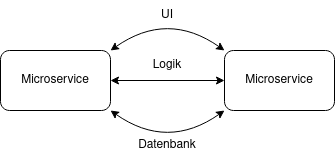
\includegraphics[width=0.60\textwidth]{figures/IntegrationMicroservices.png}
    \caption{Integration von Microservices auf verschiedenen Ebenen \parencite[vgl.][S. 167]{wolffMicroservices2018}}
\end{figure}

Auf Datenbank-Ebene können Microservices integriert werden, indem sie auf dieselbe Datenbank zugreifen. Diese Methode ist einfach zu implementieren, aber bringt jedoch Nachteile mit sich \parencite[vgl.][S. 69]{newmanMicroservices2015}. Wenn durch Änderungen in einem Microservice die Datenstruktur angepasst wird, wirkt sich das auf die anderen Microservices aus und die Unabhängigkeit wird reduziert. Auch die Technologiefreiheit wird dadurch beschränkt. Eigene Datenbanken oder zumindest Datenbankschemata erlauben so mehr Freiheiten und eine schnellere Änderung von Datenstrukturen.

Die Benutzerschnittstelle oder \ac{UI} ist die Ebene auf der alle Funktionalitäten der Microservices zusammengeführt werden. Um auch hier ein hohe Unabhängigkeit zu gewährleisten, ist es ratsam jeden Microservice mit einer UI auszustatten. Sommit könnten alle Änderungen, egal ob sie UI, Logik, oder Datenbank betreffen, von einem Entwicklerteam umgesetzt werden. Das Problem ist jedoch, dass \acp{} schnell sehr umfangreich werden und so einen Microservice unnötig groß machen. Außerdem benötigen moderne Anwendungen häufig unterschiedliche Frontends für verschiedene Gerätetypen. Deshalb werden Frontends häufig weiterhin monolithisch Aufgebaut. Mittlerweile gibt es jedoch auch immer mehr Micro-Frontends, welche den Microservice-Ansatz auf Frontends übertragen \parencite[vgl.][S. 1]{peltonenMotivations2021}.

Zuletzt können Microservices auf Logik-Ebene miteinander verbunden werden. Microservices müssen untereinander kommunizieren, wenn sie die Funktionalität eines anderen Microservices benötigen. Wichtig dabei ist, dass die Microservices trotzdem eine größtmögliche Unabhängigkeit bewahren. Zu viel Kommunikation zwischen zwei Microservices sind ein Hinweis auf eine schlechte Aufteilung \parencite[vgl.][S. 104]{wolffMicroservices2018}. Zyklische Abhängigkeiten sollten unter allen Umständen vermieden werden. Die Kommunikation läuft über \acp{API}. Eine beliebter Architekturstil für \acp{API} ist \ac{REST}. \ac{REST} vereinheitlicht die Struktur und das Verhalten von Schnittstellen \parencite[vgl.][S. 76]{fieldingArchitectural2000}. Bei einer \ac{REST}-\acp{API} gibt es eine Vielzahl von Ressourcen, die über eindeutige \acp{URI}, identifiziert werden. Die Ressourcen können über \acs{HTTP}-Anfragen mit verschiedenen \acs{HTTP}-Anfragemethoden manipuliert werden.

\subsection{Docker}

Anwendungen mit Microservice-Architektur verwenden häufig Containervirtualisierung zur Bereitstellung. Durch die leichtgewichtige Containervirtualisierung können mehrere isolierte Instanzen eines Betriebssystems auf dem selben Kernel ausgeführt werden. Dadurch sind die Container ressourcenschonender als die herkömmliche Virtualisierung mittels Hypervisor, bei dem jede virtuelle Maschine ein eigenes vollständiges Betriebssystem ausführt \parencite[vgl.][S. 166f]{newmanMicroservices2015}.

\begin{figure}[H] 
    \centering
    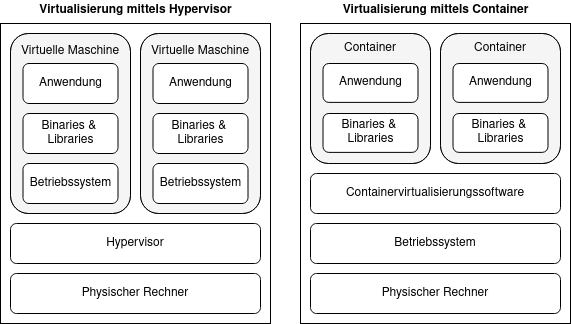
\includegraphics[width=0.95\textwidth]{figures/VergleichVirtualisierung.png}
    \caption{Vergleich Virtualisierung mittels Hypervisor und Container}
\end{figure}

Für die Ausführung einer Anwendung werden Abhängigkeiten wie zum Beispiel Bibliotheken, Compiler und Interpreter benötigt. Des Weiteren muss die Anwendung richtig konfiguriert werden. Vor allem bei einer Microservice-Architektur kann das ein Problem werden, da die Microservices über große Netzwerke verteilt auf verschiedenartigen Rechnern bereitgestellt werden sollen. Containervirtualisierung löst dieses Problem mit einem standardisierten Image-Datei, das die Anwendung mitsamt aller Abhängigkeiten und Konfigurationen beinhaltet \parencite[vgl.][S. 9]{arundelCloud2019}. Diese Image-Datei läuft unabhängig von der Plattform auf jedem Rechner, sofern die zugehörige Containervirtualisierungssoftware installiert ist.

Eine freie Software zur Containervirtualisierung ist Docker \parencite[vgl.][]{dockerinc.Docker2022}. Sie ist die beliebteste und verbreitetste Software für diesen Zweck \parencite[vgl.][S. 20]{hightowerKubernetes2018} und ergänzt die Containervirtualisierung um benutzerfreundliche Werkzeuge. Docker basiert auf der Virtualisierung mit Linux-Containern. Durch herkömmliche Virtualisierung kann Docker jedoch auch auf anderen Betriebssystemen betrieben werden. Im Folgenden werden die wichtigsten Begriffe und Funktionen von Docker näher beschrieben.

\subsubsection{Docker Image}

Ein Docker Image ist das Speicherabbild eines Containers. Das Image beinhaltet alle Informationen, die zum Starten eines Containers notwendig sind.  Bei Docker besteht das Image aus mehreren Schichten. Jede Schicht repräsentiert eine Abhängigkeit oder Konfiguration, welche für die Anwendung benötigt wird. Docker optimiert automatisch den verwendeten Speicherplatz durch Wiederverwendung, wenn zwei Images eine gleiche Schicht verwenden. Die Docker Images sind portabel. Über zentrale Registrys können die Images verwaltet, gespeichert und verteilt werden. Docker Hub ist die größte öffentliche Registry mit einer Vielzahl an Images, die von anderen Benutzern bereitgestellt werden. Beim Ausführen eines Images wird auf Basis des Images ein Container gestartet. Das Image ist wiederverwendbar und es können beliebig viele Container aus einem Image erzeugt werden. 

\subsubsection{Dockerfile}

Ein Dockerfile ist eine Textdatei mit mehreren Befehlen, die ein Docker Image beschreiben. Aus einem Dockerfile kann das entsprechende Image gebaut werden. Dazu werden die einzelnen Befehle abgearbeitet und für jeden Befehl eine neue Schicht in dem zugehörigen Image angelegt. Begonnen wird meistens mit einem Basis-Image, welches bereits vorhanden ist. Danach folgen spezifische Änderungen, damit die gewünschte Anwendung ausgeführt werden kann.

\subsubsection{Container}
Ein Container ist die aktive Instanz eines Images. Er besitzt eine begrenzte Lebensdauer und wird, nachdem der in ihm laufende Prozess abgeschlossen ist, beendet. Container sind in der Regel unveränderlich. Soll ein Container geändert werden, so wird der alte Container gegen einen neuen ausgetauscht. Jeder Container besitzt sein eigenes Dateisystem, Anteil an CPU, Speicher und Prozessraum. Er besitzt auch seine eigenen Bibliotheken, Compiler und Interpreter und ist so unabhängig von allen Softwareversionen, die auf dem eigentlichen Betriebssystem installiert sind. Lediglich der Kernel wird geteilt und bildet somit die einzige Abhängigkeit. 

\begin{figure}[H] 
    \centering
    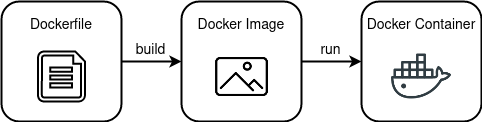
\includegraphics[width=0.8\textwidth]{figures/DockerFileImageContainer.png}
    \caption{Weg vom Dockerfile zum Container}
\end{figure}

\subsection{Kubernetes}

Wenn Microservices in Containern bereitgestellt werden, wird es schnell nicht mehr möglich, die Container manuell zu verwalten. Service Discovery, Skalierung und die Lastverteilung gestaltet sich als aufwendige Probleme. Die Open-Source-Plattform Kubernetes versucht diese Probleme zu lösen \parencite[vgl.][]{linuxfoundationKubernetes2022}. Der Name \glqq Kubernetes\grqq{} stammt aus dem griechischen und bedeutet soviel wie Steuermann. Kubernetes hilft bei der Koordination und Sequenzierung verschiedener Aktivitäten sowie bei der Verwaltung der verfügbaren Ressourcen und bei einer effizienten Lastverteilung \parencite[vgl.][S. 11]{arundelCloud2019}. Kubernetes bietet somit viele Funktionen, die die Bereitstellung von Microservices erleichtern. Häufig wird Kubernetes mit Docker verwendet, es unterstützt aber auch andere Anwendungen zur Containervirtualisierung.

\subsubsection{Aufbau}

Die größte Organisationseinheit der Plattform ist ein Kubernetes Cluster. Ein Cluster besteht aus mindestens einem Control Plane und einem Node. Der Control Plane verwaltet sämtliche Nodes. Um Ausfallsicherheit zu gewährleisten können auch mehrere Control Planes in einem Cluster betrieben werden. Ein Control Plane enthählt eine Key-Value-Datenbank namens etcd. In ihr wird die gesamte Konfiguration des Clusters gespeichert. Des Weiteren enthält der Control Plane einen \ac{API}-Server, mit der die Nodes kommunizieren. Auch externe Komponenten können mit ac{API}-Server kommunizieren und so Informationen abfragen oder das Cluster konfigurieren. Der Controller Manager steuert über den ac{API}-Server die einzelnen Nodes. Des Weiteren besitzt der Control Plane einen Scheduler, der die Last verteilt und überwacht.

In der Regel besteht ein Cluster aus vielen Nodes. Dabei kann es sich um physische Rechner aber auch um virtuelle Maschinen handeln. Auf den Nodes laufen die Container mit den eigentlichen Anwendungen. Außerdem besitzt jeder Node einen Kubelet. Dieser Kubelet kommuniziert mit dem Controller Manager und verwaltet den Status der Container auf dem jeweiligen Node.

\begin{figure}[H] 
    \centering
    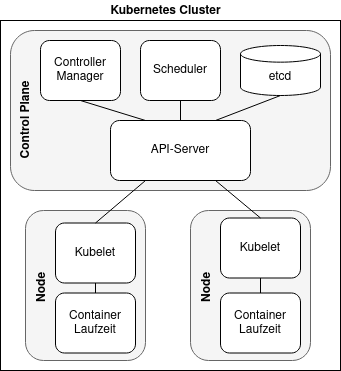
\includegraphics[width=0.75\textwidth]{figures/KubernetesCluster.png}
    \caption{Aufbau eines Kubernetes Cluster}
\end{figure}

\subsubsection{Objekte}

Kubernetes stellt eine Reihe von abstrakten Objekten zur Verfügung, mit denen der Status des Systems dargestellt wird und welche es erleichtern eine Microservice-Architektur zu bauen \parencite[vgl.][S. 13]{hightowerKubernetes2018}. Diese Objekte werden in Manifesten beschrieben. Bei den Manifesten handelt es sich üblicherweise um YAML-Dateien. Die Manifeste sind deklarativ aufgebaut, das bedeutet der gewünschte Ausgangszustand wird beschrieben. Nachdem das Manifest übergeben wurde, führt Kubernetes die entsprechenden Aktionen aus, um den beschriebenen Zustand zu erreichen.

Zu den grundlegenden Objekten gehören die Folgenden:
\begin{itemize}
\item Pods sind die kleinste einsetzbare Einheit. Ein Pod repräsentiert eine einen einzelnen Container oder eine Gruppe von Containern. Alle Container in einem Pod laufen immer auf dem gleichen Node.
\item Namespaces werden zur logischen Unterteilung des Clusters verwendet. Sie können zur Isolation verschiedener Entwicklerteams oder Anwendungsmodule genutzt werden.
\item Volumes bieten persistenten Speicher, der auch nach der Lebenszeit eines Pods bestehen bleibt.
\item ConfigMaps ermöglichen das Speichern von Konfigurationsdaten als Key-Value-Paare. Sie können beispielsweise von Pods als Umgebungsvariablen konsumiert werden.
\item Labels können anderen Objekten zugeordnet werden, um diese zu Gruppieren.
\item ReplicaSets sorgen dafür, dass eine bestimmte Anzahl von Kopien eines Pods gleichzeitig laufen zu lassen.
\item Deployments repräsentieren eine zustandslose Anwendung. Deployments verwenden ReplicaSets. Ein Deployment überwacht fortlaufend den Status der Container und kann sie beispielsweise bei Bedarf neu starten.
\end{itemize}

\begin{figure}[H] 
    \centering
    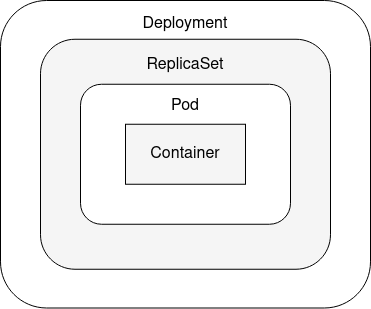
\includegraphics[width=0.55\textwidth]{figures/KubernetesDeployment.png}
    \caption{Aufbau von einem Deployment}
\end{figure}

In den nächsten Abschnitten werden noch ein paar weitere Objekte beschrieben, welche für die Service Discovery und Skalierung nützlich sind.

\subsubsection{Service Discovery}
Kubernetes ist ein dynamisches System. Ein Microservice, der in einem Pod läuft, kann schnell gestoppt, gestartet oder repliziert werden. Da auch mehrere Instanzen eines Microservices gleichzeitig laufen können, wird ein fester Enpunkt benötigt, über den gleichartige Pods erreichbar sind. In Kubernetes kann dafür ein Service-Objekt erstellt werden. Ein Service stellt eine unveränderliche virtuelle IP-Adresse bereit, welche Kubernetes per Lastverteilung auf die passenden Pods verteilt. Innerhalb des Clusters kann ein Service auch über den Service-Namen aufgerufen werden, welcher mit dem \ac{DNS} aufgelöst wird. Ein Service vom Typ ClusterIP ist von außerhalb des Clusters nicht aufrufbar. Mit dem Typ NodePort kann der Service von außen zugänglich gemacht werden. Dazu wird ein fester Port auf allen Nodes geöffnet und der Datenverkehr über diesen Port an den entsprechenden Service weitergeleitet.

\begin{figure}[H] 
    \centering
    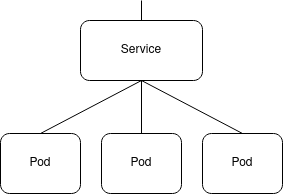
\includegraphics[width=0.55\textwidth]{figures/KubernetesService.png}
    \caption{Service als Endpunkt für eine Gruppe von Pods \parencite[vgl.][S. 67]{arundelCloud2019}}
\end{figure}

\subsubsection{Skalierung}

Über ReplicaSets lässt sich eine feste Anzahl von Kopien eines Pods festlegen. In der Praxis soll die Anzahl häufig nach der Auslastung skaliert werden. Diese Aufgabe kann Kubernetes automatisiert werden. Dafür wird das das Objekt \ac{HPA} angeboten. Mit dem \ac{HPA} kann beispielsweise eine Skalierung in Abhängigkeit der CPU-Auslastung vorgenommen werden. Des Weiteren wird in dem Objekt angegeben, wie viele Kopien mindestens vorhanden sein sollten und wie viele maximal erstellt werden dürfen. 

\subsubsection{Kubectl}

kubectl ist der offizielle Kubernetes-Client und dient der Steuerung von Kubernetes. Bei kubectl handelt es sich um ein \ac{CLI} für die Interaktion mit dem \ac{API}-Server des Control Planes. Mit kubectl können beispielsweise Objekte verwaltet werden und der Status des gesamten Clusters untersucht werden.

\subsubsection{Minikube}

Minikube ist ein Werkzeug, um ein lokales Kubernetes Cluster zu betreiben. Minikube erstellt ein Cluster bestehend aus nur einem Node in einer virtuellen Maschine. Der Node fungiert dabei sowohl als Control Plane sowie auch als Node. Minikube unterstützt mittlerweile auch den Betrieb mit mehreren Nodes. Des Weiteren kann das gesamte Cluster selbst auch in einem Docker Container anstatt in einer virtuellen Maschine betrieben werden. Minikube erstellt beim Start automatisch eine kubectl-Konfiguration, welche auf das Cluster zeigt und somit über kubectl-Befehle gesteuert werden kann. 

\clearpage
\section{Erläuterung des Fallbeispieles}
Ziel des Fallbeispieles ist es, ein Verfahren vom Entwurf bis zur Bereitstellung von containerisierten Microservices mit Kubernetes zu implementieren. Auf Basis dieses Verfahrens sollen Aussagen zur Umsetzung und dem Anwendungsgebiet getroffen werden können. Als Beispiel wird ein vereinfachtes \ac{CRM}-System verwendet. In diesem Kapitel werden die Vorgaben an das Fallbeispiel beschrieben.

\subsection{Anwendungseinsatz}
Ein \ac{CRM}-System ist eine Software für das Kundenbeziehungsmanagement. \ac{CRM}-Systeme sind komplexe betriebliche Anwendungssysteme. Durch ihre Größe und ihre vielen verwobenen Dienste gestaltet sich der Entwurf und die Weiterentwicklung häufig schwierig. \ac{CRM}-Systeme haben eine große fachliche Breite, was zu einem hohen Koordinationsaufwand bei der Entwicklung und der Bereitstellung führt \parencite[vgl.][S. 62]{trempArchitekturen2021}. Somit eignet sich ein \ac{CRM}-System als gutes Beispiel für die Umsetzung mit einer Microservice-Architektur, welche die Probleme weitgehend beheben soll. 

Das \ac{CRM}-System soll für das \ac{B2C} Umfeld entwickelt werden. Es soll bei der Verwaltung von Kontakten beziehungsweise Kunden helfen. Zu jedem Kontakt sollen Informationen und eine Historie mit allen Interaktionen abgespeichert werden. Darüber hinaus soll es auch möglich sein, Verkaufschancen zu verwalten und einem Kontakt zuzuordnen.

\subsection{Anwendungsfunktionen}
Die Kernfunktionalität des zu erstellenden \ac{CRM}-Systems ist das Anlegen, Anzeigen, Bearbeiten und Löschen von Kontakten, Interaktionen und Verkaufschancen. Konkret sollen die folgenden funktionalen Anforderungen von dem System erfüllt werden:
\begin{itemize}
\item Kontakte sollen mit Identifikationsnummer, Name, Geburtsdatum, Geschlecht, Telefonnummer, E-Mail-Adresse und Adresse angelegt, angezeigt, geändert und gelöscht werden können.
\item Interaktionen mit einem Kontakt sollen mit Identifikationsnummer, Art der Interaktion, Datum, Uhrzeit, Notizen und dem zugehörigen Kontakt angelegt, angezeigt, geändert und gelöscht werden können.
\item Mögliche Verkaufschancen sollen mit Identifikationsnummer, Status, voraussichtlichem Abschlussdatum, Verkaufswert, Rabatt, Budget des Kunden, Notizen und dem zugehörigen Kontakt angelegt, angezeigt, geändert und gelöscht werden können.
\end{itemize} 

Alle Funktionen sollen über eine einfache grafische Benutzeroberfläche mit dem Webbrowser bedienbar sein. Des Weiteren sollen alle Funktionen auch über \acp{API} angesteuert werden können, um die Integrierbarkeit mit anderen Systemen zu erleichtern. Durch die lose Kopplung einer Microservice-Architektur, soll eine flexible Skalierung und Erweiterbarkeit der Anwendung gewährleistet werden. Authentifizierung, Autorisierung und andere Sicherheitsfunktionen sollen nicht beachtet werden.

\clearpage
\section{Entwurf der Microservices}
In diesem Kapitel wird die Microservice-Architektur des \ac{CRM}-Systems entworfen. Dabei wird zuerst die Makro-Architektur des Gesamtsystems ausgearbeitet und anschließend die Mikro-Architektur der einzelnen Microservices festgelegt.

\subsection{Makro-Architektur}
Die Makro-Architektur muss besonders sorgfältig konzipiert werden, da Veränderungen auf dieser Ebene zu einem späteren Zeitpunkt sehr aufwendig werden können. Das Wichtigste ist eine gute fachliche Aufteilung der Microservices. Für die Aufteilung wird nach dem \ac{DDD} vorgegangen. Die Anwendung lässt sich in drei Bounded Contexts unterteilen: Kontaktverwaltung, Interaktionsverwaltung und Chancenverwaltung. Jeder dieser drei Bereiche besitzt ein eigenes Datenobjekt für einen Kontakt, eine Interaktion oder eine Chance. Eine Interaktion und eine Chance sollen einem Kontakt zuogeordnet werden können, deshalb benötigen diese Bounded Contexts einen Teil der Kontaktdaten. Die Identifikationsnummer eines Kontaktes reicht aus, um einer Interaktion oder Chance einen eindeutigen Kontakt zuzuordnen. Daraus ergibt sich die folgende Context Map, mit den drei Bounded Contexts und den Daten, an denen jeder Bounded Context interessiert ist. Anhand der identifizierten Kontextgrenzen wird die Anwendung in einen Kontakt-Microservice, einen Interaktions-Microservice und einen Chancen-Microservice aufgeteilt.

\begin{figure}[H] 
    \centering
    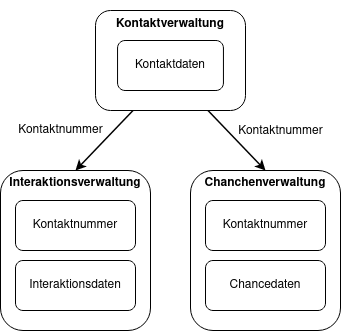
\includegraphics[width=0.60\textwidth]{figures/ContextMap.png}
    \caption{Context Map}
\end{figure}

Nachdem die fachliche Einteilung erledigt ist, kann jetzt die technischen Architektur festgelegt werden. Zur flexiblen Skalierbarkeit müssen die Microservices zustandslos sein. Alle persistenten Daten werden also in einer Datenbank abgelegt. Um eine möglichst große Unabhängigkeit zwischen den Microservices zu haben, wird jedem Microservice eine eigene Datenbank mit einem eigenen Datenbankschema zugeordnet. So können Datenstrukturen geändert werden, ohne unbeabsichtigte Auswirkungen auf andere Microservices zu haben. Der Interaktions-Microservice und der Chancen-Microservice benötigen für die Zuordnung zu einem Kontakt Informationen vom Kontakt-Microservice. Zwischen diesen Microservices ist somit eine Kommunikation nötig. Gibt es zu viele solcher Abhängigkeiten oder zyklische Aufrufe, sollte die Einteilung der Microservices überarbeitet werden. Das ist bei dieser Aufteilung jedoch nicht der Fall. Da alle Funktionalitäten auch über \acp{API} aufrufbar sein sollen, bietet es sich an, die Kommunikation zwischen den Microservices auch über diese \acp{API} abzuwickeln. Um die Microservices klein zuhalten, wird ein zentrales Frontend entwickelt werden, welches alle Funktionalitäten der Microservices bündelt. Um die Funktionalitäten zu integrieren, greift das Frontend auch auf die \acp{API} der Microservices zu. Somit ergibt sich der folgende Architekturentwurf aus drei verschiedenen Microservices mit drei zugehörigen Datenbanken und einem Frontend.

\begin{figure}[H] 
    \centering
    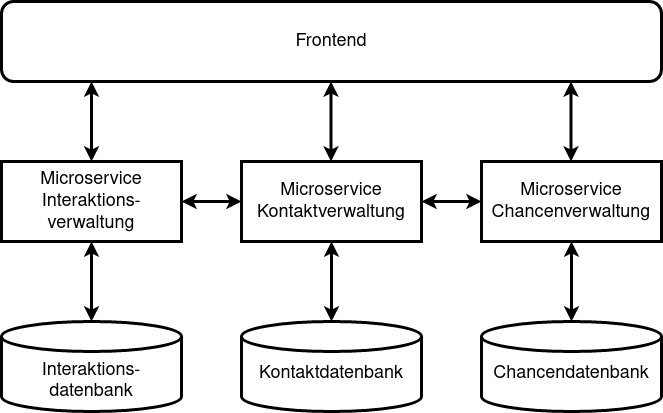
\includegraphics[width=0.8\textwidth]{figures/CRMEntwurf.png}
    \caption{Makro-Architektur des CRM-Systems}
\end{figure}

Als Nächstes müssen die \acp{API} der Microservices spezifiziert werden. Die \ac{API} wird nach dem \ac{REST}-Architekturstil entworfen. Die Kommunikation erfolgt dabei über \ac{HTTP}. Die \ac{REST}-Ressourcen sollen im \ac{JSON}-Format dargestellt werden. Für jeden Microservice werden die Endpunkte, unter der die \ac{API} aufrufbar ist und die HTTP-Anfragemethode bestimmt.

\begin{figure}[H] 
\centering
    \begin{tabularx}{\columnwidth}[H]{|p{45mm}|p{35mm}|X|}
    		\hline
        \rowcolor{lightgray!20}
        \textbf{Endpunkt} & \textbf{Methode} & \textbf{Beschreibung} \\
        \hline
        \hline
        \multicolumn{3}{|c|}{Kontakt-Microservice} \\
        \hline
        /contacts & GET & Gibt alle Kontakte zurück \\
        /contacts & POST & Fügt einen neuen Kontakt hinzu \\
        /contacts/\{ID\} & GET & Gibt einen Kontakt zurück \\
        /contacts/\{ID\} & PUT & Ändert einen Kontakt \\
        /contacts/\{ID\} & DELETE & Löscht einen Kontakt \\
        \hline
        \hline
        \multicolumn{3}{|c|}{Interaktions-Microservice} \\
        \hline
        /interactions & GET & Gibt alle Interaktionen zurück \\
        /interactions & POST & Fügt einen neue Interaktion hinzu \\
        /interactions/\{ID\} & GET & Gibt eine Interaktion zurück \\
        /interactions/\{ID\} & PUT & Ändert eine Interaktion \\
        /interactions/\{ID\} & DELETE & Löscht eine Interaktion \\
        \hline
        \hline
        \multicolumn{3}{|c|}{Chancen-Microservice} \\
        \hline
        /opportunity & GET & Gibt alle Chancen zurück \\
        /opportunity & POST & Fügt einen neue Chance hinzu \\
        /opportunity/\{ID\} & GET & Gibt eine Chance zurück \\
        /opportunity/\{ID\} & PUT & Ändert eine Chance \\
        /opportunity/\{ID\} & DELETE & Löscht eine Chance \\
        \hline
    \end{tabularx}
    \caption{Entwurf der REST-API}
\end{figure}

Service Discovery und Lastverteilung muss das System nicht selbst erledigen. Diese Funktionen werden von Kubernetes übernommen und erst bei der Bereitstellung konfiguriert.

\subsection{Mikro-Architektur}
Für das Gesamtsystem ist die Architektur eines einzelnen Microservice nicht von Bedeutung. Dadurch besitzt man bei der Gestaltung der Mikro-Architektur und vor allem bei der Auswahl des Technologie-Stacks viele Freiheiten. In diesem Fallbeispiel werden ausschließlich bewährte und beliebte Technologien eingesetzt. Die drei Microservices werden mit demselben Technologie-Stack und mit einer gleichartigen Architektur entworfen, um den Entwicklungsaufwand zu reduzieren. Es wäre aber auch möglich, alle Microservices mit verschiedenen Technologien zu implementieren, solange sie die gewünschten Schnittstellen anbieten können. Es wird Java in Verbindung mit dem Spring Boot Framework verwendet. Spring Boot bietet ein einsatzfertiges Baugerüst für Java-Anwendungen und eine einfache Auswahl von benötigten Abhängigkeiten, wie beispielsweise Datenbanktreibern. Auch \ac{REST}-\acp{API} werden von Spring Boot unterstützt. Spring Boot ist der De-Facto-Standard für Microservices in Java \parencite[vgl.][]{vmwareinc.Spring2022}. Für die Datenbanken wird MongoDB verwendet. MongoDB ist ein modernes dokumentorientiertes Datenbankmanagementsystem  \parencite[vgl.][]{mongodbinc.MongoDB2022}. Daten werden in Collections als Dokumente mit einem \ac{JSON}-ähnlichen Aufbau verwaltet. Die Datenstrukturen sind flexibel und können leichter umstrukturiert werden als bei klassischen Datenbanken. MongoDB wird auch als NoSQL-Datenbank bezeichnet.

Für alle drei Microservices werden Domänenmodelle erstellt. Die Domänenmodelle enthalten alle fachlichen Entitäten sowie deren Eigenschaften und Beziehungen. Für die Modellierung wird ein Klassendiagramm nach der \ac{UML} verwendet \parencite[vgl.][]{Unified2017}. \ac{UML} ist eine grafische Modellierungssprache, welche im Laufe der Arbeit noch häufiger eingesetzt wird. Die Domänenmodelle enhalten die gewünschten Eigenschaften aus den Anforderungen. Beim Kontakt-Microservice besteht das Datenmodell aus zwei Entitäten. Ein Kontakt besteht aus einer Adresse und mehreren anderen Eigenschaften, wie dem Namen, dem Geburtsdatum und einer Mail-Adresse. Da MongoDB eine NoSQL-Datenbank ist, besitzen die beiden Entitäten keine relationale Beziehung. Die Adresse wird verschachtelt im MongoDB-Dokument vom Kontakt abgespeichert werden. Des Weiteren enthält das Modell zwei Enumerationen für Auswahl des Geschlechts und der Nationalität.

\begin{figure}[H] 
    \centering
    \includegraphics[width=0.9\textwidth]{figures/DomänenmodellKontakt.png}
    \caption{Domänenmodell für den Kontakt-Microservice}
\end{figure} 

Das Datenmodell vom Interaktions-Microservice besteht lediglich aus einer einzelnen Entität und einer Enumeration für die Interaktionsart.

\begin{figure}[H] 
    \centering
    \includegraphics[width=0.9\textwidth]{figures/DomänenmodellInteraktion.png}
    \caption{Domänenmodell für den Interaktions-Microservice}
\end{figure}

Der Chancen-Microservice ist ähnlich aufgebaut und besitzt neben einer einzelnen Entität eine Enumeration für den Status einer Verkaufschance.

\begin{figure}[H] 
    \centering
    \includegraphics[width=0.9\textwidth]{figures/DomänenmodellChance.png}
    \caption{Domänenmodell für den Chancen-Microservice}
\end{figure}

Die einzelnen Microservices werden nach einer hexagonalen Architektur entworfen. Dabei handelt es sich um ein Architekturmuster bei der die Logik im Mittelpunkt steht. Sie hat verschiedene Schnittstellen (Ports), welche mit diversen Adaptern benutzt werden können. Das Architekturmuster wird deshalb auch als Ports and Adapters bezeichnet. Eine hexagonale Architektur ist eine Weiterentwicklung der klassischen Drei-Schichten-Architektur, bei der die Anwendung in eine Präsentationsschicht, eine Logikschicht und eine Datenhaltungsschicht aufgeteilt wird.

\begin{figure}[H] 
    \centering
    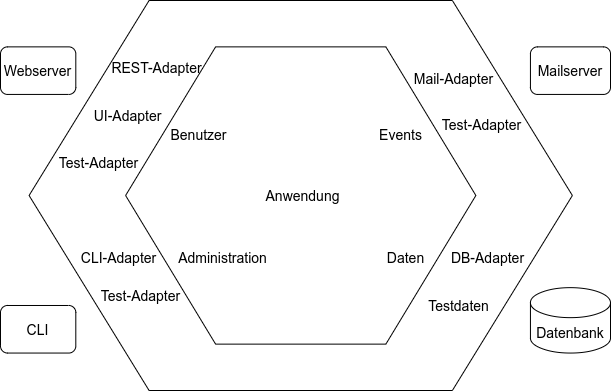
\includegraphics[width=0.9\textwidth]{figures/HexagonalDesignConcept.png}
    \caption{Überblick einer hexagonalen Architektur \parencite[vgl.][S. 204]{wolffMicroservices2018}}
\end{figure}

Jede Facette der Anwendung, wie Benutzer, Daten oder Admin ist ein Port, welcher von den Adaptern auf Technologien wie \ac{REST} umgesetzt wird \parencite[vgl.][S. 204]{wolffMicroservices2018}. Die Logik der Anwendung wird klar abgetrennt und nur die Adapter ermöglichen eine Kommunikation nach Außen. Dadurch bleibt der fachliche Code unabhängig vom technischen Code. Für das Fallbeispiel wird lediglich ein Port für die Daten und ein Port für die Benutzung benötigt. Zusätzlich wird ein Adapter für die \ac{REST}-\ac{API} und ein Adapter für MongoDB benötigt.

Als Frontend wird eine clientseitige Webanwendung eingesetzt. Diese wird mithilfe der JavaScript-Bibliothek React implementiert. React ist die beliebteste Bibliothek zum Erstellen von Web-\acp{UI} \parencite[vgl.][]{stackoverflowMost2021}. Anwendungen werden dabei aus wiederverwendbaren Komponenten zusammengesetzt werden, welche effizient gerendert und aktualisiert werden. Die Komponenten können sowohl aus JavaScript, \ac{HTML} und \ac{CSS} bestehen. 

\clearpage
\section{Implementierung}
In diesem Kapitel wird der erstellte Entwurf implementiert. Zuerst werden die Microservices angefertigt und anschließend das Frontend. Es sei auch erwähnt, dass der vollständige Quellcode unter dem folgenden GitHub Repository einsehbar ist: \href{https://github.com/SimonHirner/bachelor-thesis}{github.com/SimonHirner/bachelor-thesis}.

\subsection{Microservices}
Die Umsetzung aller drei Microservices ist sehr ähnlich, deshalb wird die Implementierung hauptsächlich am Beispiel des Kontakt-Microservices erläutert. Als Erstes wird das erstellte Domänenmodelle für den Kontakt-Microservice implementiert. Jede Entität wird mit seinen Eigenschaften wird in Java als eine Klasse mit Attributen dargestellt. Die Endpunkte der spezifizierten \ac{REST}-\ac{API} werden in der Klasse ContactController erstellt. Dieser fungiert als ein Adapter im Sinne der hexagonalen Architektur. Er benötigt einen Port, mit dem er auf Funktionen der Geschäftslogik zugreifen kann. Dafür wird das Interface ContactService erstellt. Dieses definiert die Funktionalitäten der Geschäftslogik, implementiert sie aber noch nicht. Erst in der Klasse ContactServiceImpl wird das Interface implementiert und die eigentliche Geschäftslogik niedergeschrieben. Dadurch ist die Logik vom Controller, der sich um die Anfragen auf die REST-Schnittstelle kümmert, unabhängig. Einen Adapter für die Anbindung an MongoDB bringt Spring bereits mit. Es muss lediglich noch das Interface ContactRepository erstellt werden, welches als Port den Adapter mit der Geschäftslogik verbindet. Die Klassen ContactController und ContactServiceImpl werden vollständig im \nameref{anhang} aufgelistet.

\begin{figure}[H] 
    \centering
    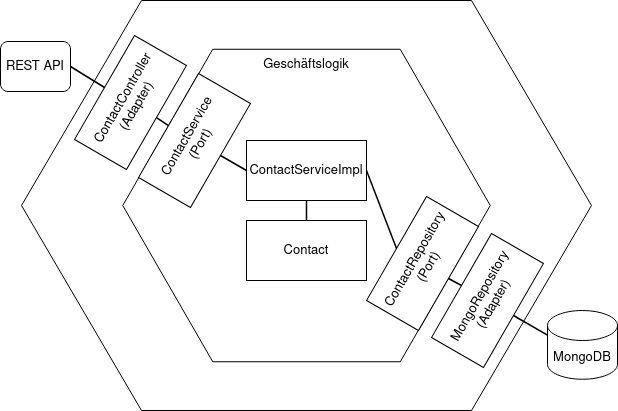
\includegraphics[width=0.9\textwidth]{figures/HexagonalDesign.png}
    \caption{Implementierung der hexagonalen Architektur beim Kontakt-Microservice}
\end{figure}

Den Mittelpunkt des Microservices bildet die Klasse ContactServiceImpl. Sie enthählt den Code, der die Geschäftslogik beschreibt. Die Klasse enthält verschiedene Methoden, um Kontakte zurückzugeben, zu löschen, zu speichern und zu ersetzen.

\begin{figure}[H] 
    \centering
    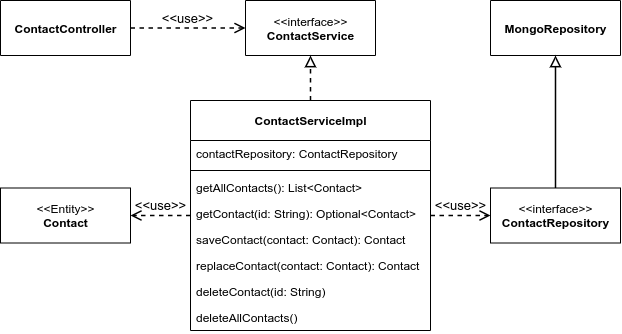
\includegraphics[width=0.9\textwidth]{figures/UMLKlassenDiagrammKontakt.png}
    \caption{Struktur vom Kontakt-Microservice}
\end{figure}

Der Interaktions-Microservice und der Chancen-Microservices unterscheiden sich bei der Geschäftslogik vom Kontakt-Microservice. Der Interaktions-Microservice muss beim Speichern einer Interaktion überprüfen, ob die Kontaktidentifikationsnummer der Interaktion gültig ist. Dafür ruft der Interaktions-Microservice den Kontakt-Microservice über seine \ac{REST}-\ac{API} auf und testet, ob zu der angegebenen Kontaktidentifikationsnummer ein Kontakt vorhanden ist. Das folgende \ac{UML}-Sequenzdiagramm zeigt den zeitlichen Verlauf der \ac{API}-Anfragen und die involvierten \ac{API}-Endpunkte. Da bei einer Chance auch eine Kontaktidentifikationsnummer angegeben werden kann, wird beim Chancen-Microservice dieselbe Logik implementiert.

\begin{figure}[H] 
    \centering
    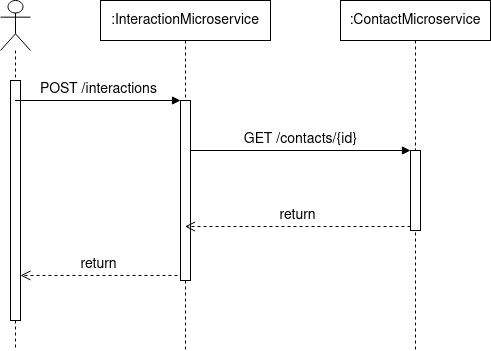
\includegraphics[width=0.75\textwidth]{figures/UMLSequenzdiagramm.png}
    \caption{Kommunikationsablauf zwischen Interaktions-Microservice und Kontakt-Microservice}
\end{figure}

Des Weiteren wird Swagger in die Microservices integriert. Bei Swagger handelt es sich ein Werkzeug zur sprachunabhängigen Spezifikation von \acp{API} \parencite[vgl.][]{smartbearsoftwareSwagger2022}. Swagger kann durch eine Abhängigkeit unkompliziert zu Spring Boot hinzu gefügt werden. Es erstellt automatisch eine Webseite mit einer Dokumentation der \ac{REST}-\ac{API}. 

\begin{figure}[H] 
    \centering
    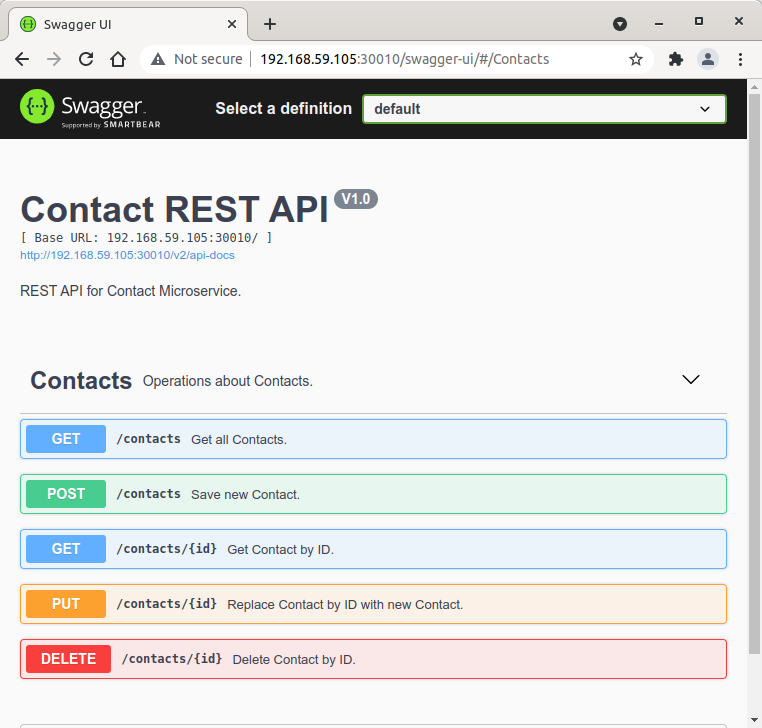
\includegraphics[width=0.9\textwidth]{figures/KontaktAPISwagger.png}
    \caption{Swagger Dokumentation der Kontakt-API}
\end{figure}

Alle drei Microservices benötigen die Adresse ihrer Datenbank, um mit ihr eine Verbindung aufzubauen. Der Interaktions-Microservice und der Verkaufschancen-Microservice brauchen darüber hinaus die Adresse des Kontakt-Microservices, um mit diesem zu kommunizieren. Diese Verbindungsinformationen werden den Anwendungen über Umgebungsvariablen übergeben. Später bei der Bereitstellung können so die Umgebungsvariablen der Container mit den richtigen Adressen besetzt werden.

\subsection{Frontend}

Das Frontend besteht aus insgesamt zehn verschiedenen Webseiten. Für jeden Kontakt, jede Interaktion und jede Verkaufschance gibt es jeweils eine Seite zum Einsehen aller Objekte, eine Seite zum Einsehen sowie Bearbeiten eines Objektes und eine Seite zum Anlegen eines neuen Objektes. Dazu hat das Frontend noch eine Startseite. Die Seiten setzen sich auch verschiedenen wiederverwendbaren Komponenten, wie beispielsweise der Navigationsleiste, Formularen und Tabellen zusammen. Die \ac{API}-Aufrufe werden über Funktionen in Service-Klassen implementiert, die von den Komponenten aufgerufen werden. Daraus ergibt sich der folgenden Aufbau für das Frontend.

\begin{figure}[H] 
    \centering
    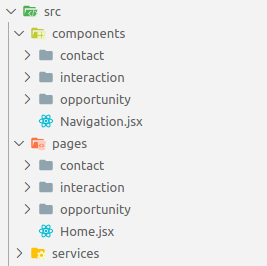
\includegraphics[width=0.5\textwidth]{figures/AufbauFrontend.png}
    \caption{Aufbau des Frontends}
\end{figure}

Zum Styling der Anwendung wird das CSS-Framework Bootstrap verwendet. Bei der Erstellung oder Bearbeitung einer Chance oder Interaktion kann über eine Dropdown-Liste ein zugehöriger Kontakte ausgewählt werden. Bei der Detailansicht eines Kontaktes wird neben den Attributen auch die zugehörigen Interaktionen und Verkaufschancen angezeigt. Im \nameref{anhang} finden sich Bildschirmfotos der beschriebenen Seiten. Auch ist dort eine der Service-Klassen zu finden, welche die Anfragen auf den Kontakt-Microservice regelt. Das Frontend benötigt die Adresse aller Services. Auch hier werden die Verbindungsinformationen über eine Umgebungsvariable übergeben. Bei React werden Umgebungsvariablen in die Datei .env.production geschrieben, da der Code des Frontends clientseitig ausgeführt wird.

\clearpage
\section{Bereitstellung mit Kubernetes}

Im letzten Teil des Fallbeispieles wird das fertige \ac{CRM}-System mit Kubernetes bereitgestellt. Dafür wird Docker, Minikube und Kubectl benötigt.

\subsection{Containerisierung}

Um die Microservices und das Frontend in Pods in einem Kubernetes Cluster laufen zu lassen, müssen sie erst mit Docker containerisiert werden. Dazu wird als Erstes ein Dockerfile für jeden Microservice erstellt. Anschließend kann aus dem Dockerfile ein Docker Image gebaut werden, mit dem dann ein entsprechender Container gestartet werden kann.

Dockerfiles besitzen eine eigene Syntax. Ein großgeschriebener Befehl wird gefolgt von einem oder mehreren Parametern. Es ähnelt einer Anleitung, welche Schritt für Schritt abgearbeitet wird. Die Dockerfiles der Microservices haben alle einen analogen Aufbau. Der erste Befehl in den Dockerfiles bestimmt, auf welchem Docker Image das neue Image basieren soll. Für die Microservices wird ein Image mit einer Java-Plattform verwendet, welches automatisch aus dem öffentlichen DockerHub heruntergeladen wird. Anschließend wird die \acs{JAR}-Datei der Anwendung in das Image kopiert. Als letzter Befehl wird festgelegt, dass die \acs{JAR}-Datei beim Start des Containers ausgeführt werden soll.

\begin{lstlisting}[language=dockerfile, caption=Dockerfile für den Kontakt-Microservice]
FROM openjdk:11-jdk-slim
ARG JAR_FILE=target/*.jar
COPY ${JAR_FILE} app.jar
EXPOSE 8080
ENTRYPOINT ["java","-jar","/app.jar"]
\end{lstlisting}

Das Frontend benötigt ein eigenes Dockerfile. Dieses hat einen mehrstufigen Aufbau. In der ersten Stufe, der Build-Stage, wird die React-Anwendung gebaut. Um die fertig gebaute Webanwendung an einen Browser auszuliefern wird ein Webserver benötigt. Die zweite Stufe des Dockerfiles basiert auf einem Image mit dem Webserver Nginx. Die React-Anwendung aus der Build-Stage wird nun in das finale Image kopiert.

\begin{lstlisting}[language=dockerfile, caption=Dockerfile für das Frontend]
FROM node:alpine as build
WORKDIR /app
COPY package*.json ./
RUN npm install --silent
COPY . .
RUN npm run build

FROM nginx:alpine
WORKDIR /usr/share/nginx/html
RUN rm -rf ./*
COPY --from=build /app/build .
ENTRYPOINT ["nginx", "-g", "daemon off;"]
\end{lstlisting}

Für die Datenbanken müssen keine eigenen Dockerfiles erstellt werden. Hier reichen unveränderte Images aus, welche vom DockerHub heruntergeladen werden können. Mit dem folgenden Befehl kann aus den erstellten Dockerfiles nun ein Docker Image gebaut werden.

\begin{lstlisting}[language=bash, caption=Docker-Befehl für das Bauen eines Images, captionpos=b]
docker build -t contact-microservice:latest .
\end{lstlisting}

\subsection{Bereitstellung}

Die fertigen Images können jetzt eingesetzt werden. Dazu wird zuerst das Kubernetes Cluster mit Minikube gestartet. Anschließend werden YAML-Dateien erstellt, in denen die gewünschten Kubernetes Objekte beschrieben werden. Für alle drei Microservices, alle drei Datenbanken und das Frontend muss jeweils ein Service und ein Deployment erstellt werden. In den Deployment-Objekten wird der Name der zuvor gebauten Images angegeben. Mit dem Attribut Replicas kann zudem die Anzahl der Pods, welche von einem Microservice gleichzeitig laufen sollen verändert werden. Bei den Microservices wird zudem die Adresse, unter der die Datenbank erreichbar ist, als Umgebungsvariable übergeben. Als Adresse wird der Name vom Service-Objekt der entsprechenden Datenbank verwendet werden.

\begin{lstlisting}[language=YAML, caption=Deployment-Objekt vom Kontakt-Microservice]
apiVersion: apps/v1
kind: Deployment
metadata:
  name: contact-service
spec:
  replicas: 1
  template:
    metadata:
      labels:
        app: contact-service
    spec:
      containers:
        - name: contact-service
          image: contact-microservice:latest
          imagePullPolicy: IfNotPresent
          ports:
          - containerPort: 8080
          env:
            - name: MONGODB_HOST
              value: contact-service
              valueFrom:
                configMapKeyRef:
                  name: contact-db-config  
                  key: host
\end{lstlisting}

Die Service-Objekte der Datenbanken sind vom Typ ClusterIP, da sie nur innerhalb des Clusters aufgerufen werden.
Die Service-Objekte der Microservices sind dagegen vom Typ NodePort. Somit kann ein fester Port angegeben werden, unter dem der Service auch von außerhalb des Clusters erreichbar ist. Anfragen auf einen Service werden automatisch von Kubernetes auf die Pods, welche dem Service zugeordnet sind, verteilt. 

\begin{lstlisting}[language=YAML, caption=Service-Objekt vom Kontakt-Microservice, captionpos=b]
kind: Service
apiVersion: v1
metadata:
  name: contact-service
spec:
  selector:
    app: contact-service
  ports:
  - protocol: TCP
    port: 8080
    nodePort: 30010
  type: NodePort
\end{lstlisting}

Sämtliche erstellte YAML-Dateien müssen über einen Kubectl-Befehl auf das Cluster angewendet werden. Kubernetes arbeitet dann automatisch die nötigen Schritte, um die beschriebenen Objekte zu erstellen.

\begin{lstlisting}[language=bash, caption=Kubectl-Befehl für das Anwenden einer YAML-Datei, captionpos=b]
kubectl apply -f contact-microservice.yaml
\end{lstlisting}

\subsection{Skalierung}
Um die Vorteile von der Microservices auszunutzen, soll die Anzahl der gleichzeitig laufenden Pods eines Microservices flexibel verwaltet werden. Abhängig von der Auslastung soll so eine horizontale Skalierung vorgenommen werden. Auch dafür wird eine YAML-Datei erstellt, in der ein \ac{HPA}-Objekt für jeden Microservice beschrieben wird. In der Datei wird angegeben, welches Deployment skaliert werden soll. Als Metrik für die Skalierung, wird die CPU-Auslastung des Pods verwendet. Darüber hinaus wird angegeben wie viele Pods vom entsprechenden Microservice minimal und maximal ausgeführt werden sollen.

\begin{lstlisting}[language=YAML, caption=HPA-Objekt vom Kontakt-Microservice, captionpos=b]
apiVersion: autoscaling/v1
kind: HorizontalPodAutoscaler
metadata:
    name: contact-service
spec:
    scaleTargetRef:
        apiVersion: apps/v1
        kind: Deployment
        name: contact-service
    minReplicas: 2
    maxReplicas: 4
    targetCPUUtilizationPercentage: 80
\end{lstlisting}

Nun ist die Bereitstellung abgeschlossen. Minikube bietet ein browserbasiertes Dashboard an, mit dem der Status des Clusters auch grafisch überprüft werden kann. Ein Bildschirmfoto des Dashboards kann im \nameref{anhang} gefunden werden. Das folgende Verteilungsdiagramm zeigt das Ergebnis der durchgeführten Bereitstellung.

\begin{figure}[H] 
    \centering
    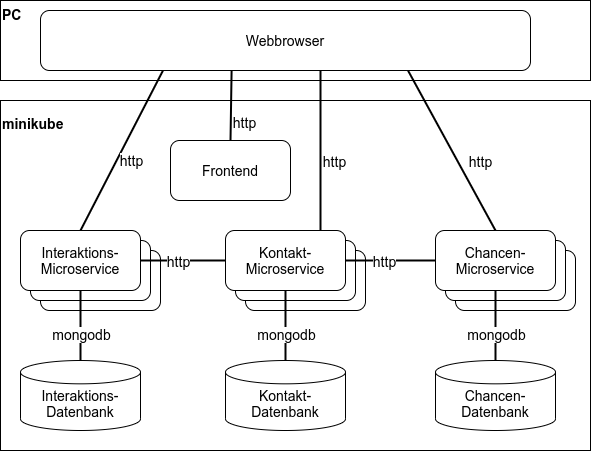
\includegraphics[width=0.82\textwidth]{figures/Verteilungsdiagramm.png}
    \caption{Verteilungsdiagramm}
\end{figure}


\clearpage
\section{Schlussbetrachtung}

Lorem ipsum dolor sit amet, consetetur sadipscing elitr, sed diam nonumy eirmod tempor invidunt ut labore et dolore magna aliquyam erat, sed diam voluptua. At vero eos et accusam et justo duo dolores et ea rebum. Stet clita kasd gubergren, no sea takimata sanctus est Lorem ipsum dolor sit amet. \\

Lorem ipsum dolor sit amet, consetetur sadipscing elitr, sed diam nonumy eirmod tempor invidunt ut labore et dolore magna aliquyam erat, sed diam voluptua. At vero eos et accusam et justo duo dolores et ea rebum. Stet clita kasd gubergren, no sea takimata sanctus est Lorem ipsum dolor sit amet.

\clearpage
\pagenumbering{Roman}
\setcounter{page}{5}
\thispagestyle{plain}
\printbibheading
\printbibliography[type=book, heading=subbibliography, title={Bücher}]
\printbibliography[type=article, heading=subbibliography,title={Artikel}]
\printbibliography[type=report, heading=subbibliography,title={Berichte}]
\printbibliography[type=inproceedings, heading=subbibliography,title={Konferenzpapier}]
\printbibliography[type=online, heading=subbibliography,title={Online}]
\printbibliography[nottype=online, nottype=article, nottype=book, nottype=report, nottype=inproceedings, heading=subbibliography, title={Sonstige}]

\clearpage
\thispagestyle{plain}
\section*{Selbstständigkeitserklärung\markboth{Selbstständigkeitserklärung}{}}
\addcontentsline{toc}{section}{Selbstständigkeitserklärung}

Hiermit erkläre ich, dass ich die vorliegende Bachelorarbeit selbständig verfasst, noch
nicht anderweitig für Prüfungszwecke vorgelegt, keine anderen als die angegebenen Quellen
oder Hilfsmittel benützt sowie wörtliche und sinngemäße Zitate als solche gekennzeichnet habe.

München, den \today
\begin{figure}[H] 
  
\includegraphics[width=0.17\textwidth]{logos/signature.png}
\end{figure}


\clearpage
\thispagestyle{plain}
\appendix

\end{document}